\section{Laufzeit}
\label{sec:laufzeit}

\subsection{Modellinferenz}

Die Laufzeiten wurden mit Batchgröße 1 auf einer Tesla V100-SXM3-32GB gemessen (Tabelle~\ref{tab:inference-runtime}). Die Messung umfasst die Modellpipeline einschließlich Datenverarbeitung und Voxelisierung auf bereits vorbereiteten Ansichtsdaten.

\begin{table}[H]
\centering
\begin{tabular}{cccc}
\toprule
\textbf{Ansicht} & \textbf{Durchsatz} & \textbf{Zeit pro Frame} & \textbf{Typische Punktzahl} \\
\midrule
merged & 11{,}7\,fps & 85\,ms & ca. 210.000 \\
os0    & 22{,}3\,fps & 45\,ms & ca. 105.000 \\
os1    & 23{,}5\,fps & 43\,ms & ca. 105.000 \\
\bottomrule
\end{tabular}
\caption{Modellinferenz-Laufzeiten auf Tesla V100-SXM3-32GB (Batchgröße 1).}
\label{tab:inference-runtime}
\end{table}

Bei einer Sensorfrequenz von 10\,Hz steht pro Frame ein Budget von 100\,ms zur Verfügung. Die Modellinferenz auf der bereits fusionierten Punktwolke bleibt mit 85\,ms darunter und lastet das Budget zu 85 Prozent aus; die Einzelsensoransichten benötigen weniger als die Hälfte (Abbildung~\ref{fig:inferenzzeit-budget}). Daraus folgt aber nur, dass die Modellinferenz 10-Hz-fähig ist.

\begin{figure}[H]
\centering
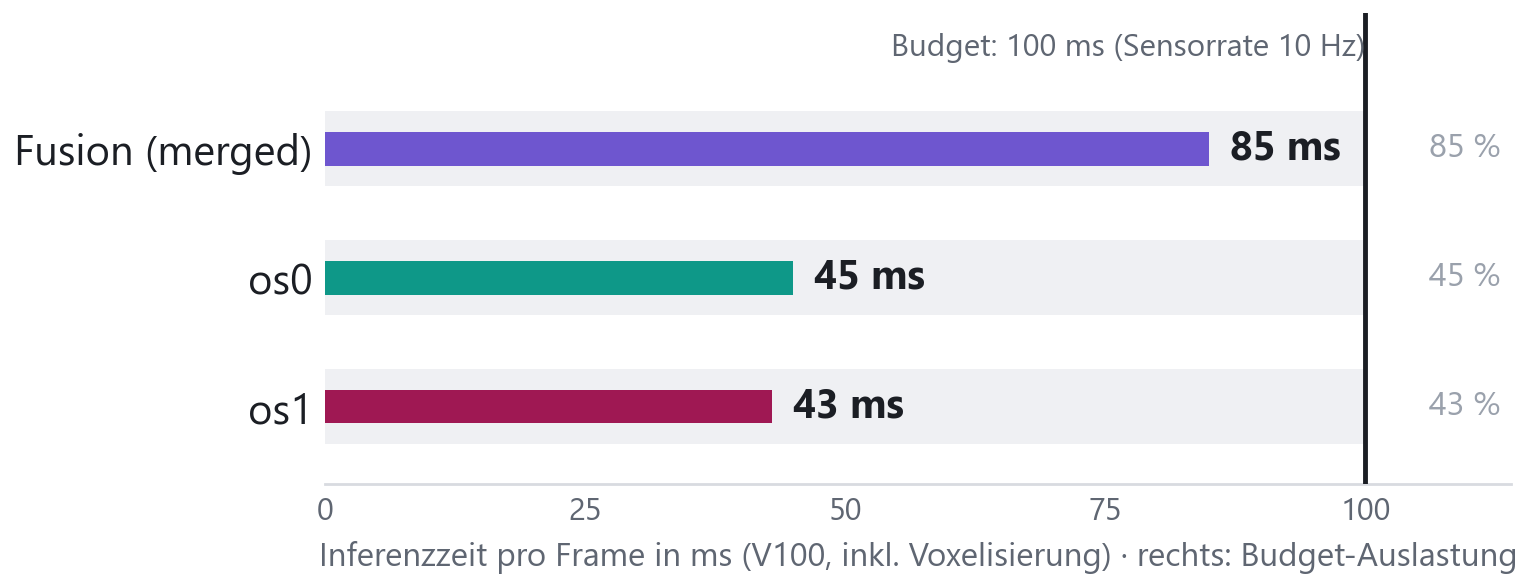
\includegraphics[width=0.95\textwidth]{images/inferenzzeit-budget.png}
\caption[Inferenzzeit im Verhältnis zum 100-ms-Budget]{Inferenzzeit je Frame im Verhältnis zum 100-ms-Budget einer 10-Hz-Sensorrate.}
\label{fig:inferenzzeit-budget}
\end{figure}

\subsection{Merge-Zeit und Ende-zu-Ende-Einordnung}

Die vorhandene Offline-Merge-Pipeline wurde auf einer lokalen CPU mit acht parallelen Workern gemessen. Die Messung umfasst 3.327 Frames, also alle verarbeiteten Rohframes und nicht nur die 2.122 Zeitstempel, die nach der Schnittmengenbildung über alle drei Ansichten für die Cross-Validation verbleiben. Über diese 3.327 Frames beträgt die mediane Bearbeitungszeit 2{,}25\,s pro Frame, der Mittelwert 2{,}20\,s, das Minimum 0{,}71\,s und das Maximum 4{,}00\,s. Enthalten sind PCD-Laden, statistischer Filter, feste Vorabtransformation, Downsampling, Normalenschätzung und per-Frame-ICP; die Registrierung dominiert die Zeit.

Es handelt sich um Einzelmessungen je Frame innerhalb eines Workers und nicht um eine aus der Gesamtlaufzeit abgeleitete Durchsatzkennzahl. Nur unter dieser Lesart lässt sich die Zahl im folgenden Absatz zu einer seriellen Latenz addieren. Dass der Median geringfügig über dem Mittelwert liegt, ist mit dieser Verteilung vereinbar: Die Zeiten sind nach unten hin gestreckt, das Minimum liegt 1{,}5\,s unter dem Median, das Maximum nur 1{,}75\,s darüber.

Der Wert ist stark hardwareabhängig. Die Vorgängerarbeit \cite{pagel2025railway} hat dieselbe Merge-Pipeline auf einer Server-CPU mit 72 Kernen gemessen und kam auf ungefähr 0{,}5\,s pro Frame. Die 2{,}25\,s sind damit keine inhärente Eigenschaft des Fusionsansatzes.

Würde diese Pipeline unverändert seriell vor der Inferenz ausgeführt, läge die Ende-zu-Ende-Latenz grob bei:

\begin{equation*}
    2{,}25\,\text{s Merge} + 0{,}085\,\text{s Inferenz} \approx 2{,}34\,\text{s pro Frame}
\end{equation*}

Das wäre nicht echtzeitfähig. Bei fest installierten Sensoren kann die Extrinsik jedoch einmalig offline bestimmt werden. Online wären dann nur Zeitsynchronisation, feste Transformation und Konkatenation erforderlich. Dieser optimierte Pfad wurde bislang nicht implementiert und gemessen.

Nach der \texttt{merged}-Inferenz verbleiben in einer seriellen 10-Hz-Pipeline nur ungefähr 15\,ms für Merge und sonstigen Overhead. Eine parallele CPU-/GPU-Pipeline könnte den Durchsatz verbessern, die Ende-zu-Ende-Latenz muss dennoch separat erfasst werden. Die korrekte Aussage ist deshalb:

\begin{quote}
    Die Modellinferenz auf bereits fusionierten Daten ist 10-Hz-fähig; die Echtzeitfähigkeit des vollständigen Online-Fusionssystems ist noch nicht nachgewiesen.
\end{quote}
